Implement fuzzy-cmeans from scratch

The paper this will be implemented from is titled, \textit{A Survey of Clustering Algorithms for Big Data: Taxonomy and Empirical Analysis}


From reference [1], the FCM algorithm is defined as follows: \newline

\begin{tcolorbox}
FCM pseudo-code:  \newline
Input: Given the dataset, set the desire number of clusters c, the fuzzy parameter m (a constant $> 1$), and the stopping condition, initialize the fuzzy partition matrix, and set stop = false.  \newline
Step 1. Do:  \newline
Step 2. Calculate the cluster centroids and the objective value J.\newline
Step 3. Compute the membership values stored in the matrix.  \newline
Step 4. If the value of J between consecutive iterations is less than the stopping condition, then stop = true.  \newline
Step 5. While (!stop)  \newline
Output: A list of c cluster centres and a partition matrix are produced.   
\end{tcolorbox}  

The equations that are used in the FCM algorithm are defined as follows: \newline

\begin{equation}
\label{eq:vk}
v_{k}=\frac{\sum_{i=1}^n{{\mu^{m}_{{i}{k}}{{\underline{p_{i}}}}}}}{\sum_{i=1}^n{{\mu^{m}_{{i}{k}}}}}
\end{equation}
   
\begin{equation}
\label{eq:distance}     
{\vert{\underline{p_{i}}}-{\underline{v_{k}}}\vert}=\sqrt{\sum_{i=1}^{n}{({\underline{x_{i}}}-{\underline{v_{k}}})^2}}
\end{equation}
  
\begin{equation}
\label{eq:objective_function}
J=\sum_{i=1}^{n}{\sum_{k=1}^{c}{\mu^{m}_{{i}{k}}{\vert{\underline{p_{i}}}-{\underline{v_{k}}}\vert^{2}}}}
\end{equation}  

\begin{equation}
\label{eq:membership_value}
{\mu^{m}_{{i}{k}}}=\frac{1}{\sum_{l=1}^{c}{(\frac{{\vert{\underline{p_{i}}}-{\underline{v_{k}}}\vert^{2}}}{{\vert{\underline{p_{i}}}-{\underline{v_{l}}}\vert^{2}}})}^{\frac{2}{m-1}}}
\end{equation}

The first step in the psuedocode sets up a loop to run until the stop condition is met. 
The stop condition is met when the value of J between consecutive iterations is less than the stopping condition. 
The second step in the psuedo code requires generating a random $\mu$ matrix, 
then calculating the cluster centroids from eq.~\ref{eq:vk} and the objective value J from eq.~\ref{eq:objective_function}. 
The third step in the psuedo code requires calculating the membership values from eq.~\ref{eq:membership_value}. 
The fourth step in the psuedo code requires checking the value of J between consecutive iterations. 
If the value of J between consecutive iterations is less than the stopping condition, then stop = true. 
The fifth step in the psuedo code requires looping back to step 2. 
The output of the psuedo code is a list of c cluster centres and a partition matrix. \newline
\begin{figure}[H]
    \centering    
    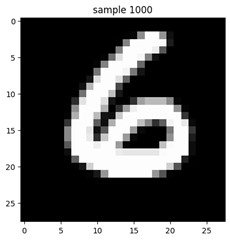
\includegraphics[width=0.5\textwidth]{image1.png}
    \caption{Handwriting Sample 1000}
    \label{fig:image1}    
\end{figure}


\begin{figure}[H]
    \centering
    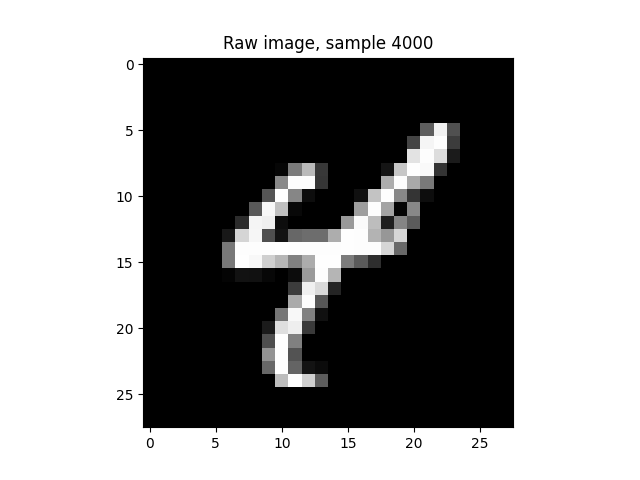
\includegraphics[width=0.5\textwidth]{image2.png}
    \caption{Handwriting Sample 4000}
    \label{fig:image2}    
\end{figure}

An example of two handwriting samples is shown as images in Figure~\ref{fig:image1} and Figure~\ref{fig:image2}. 
These images were produced using the `imshow' function from the `matplotlib' Python library.

Our group independently implemented the FCM algorithm in python then compared results among the group members. After comparison of results, we determined corrected issues where necessary. The final implmentation of the FCM code has been attached via D2L in an appropriately named Jupyter notebook.

The FCM algorithm was ran against two versions of the skewed MNIST dataset.
The first version retained the 784 dimensions, while a second version utilized principal component analysis to reduce the dimensionality of the dataset to 2 dimensions. 
The results of the FCM algorithm were compared to the actual labels of the dataset using the rand index.
The rand index is a value between 0 and 1. 
A value of 1 indicates that the clusters are identical to the labels.
A value of 0 indicates that the clusters are completely different from the labels. 
The rand index is a good measure of the accuracy of the clustering algorithm.




%\begin{center}
%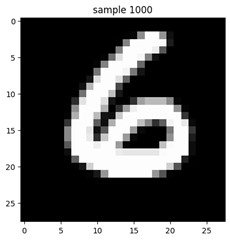
\includegraphics[width=0.35\textwidth]{image1.png}
%\captionof{figure}{Handwriting Sample 1000\label{fig:image3}}
%\end{center}

%\begin{center}
%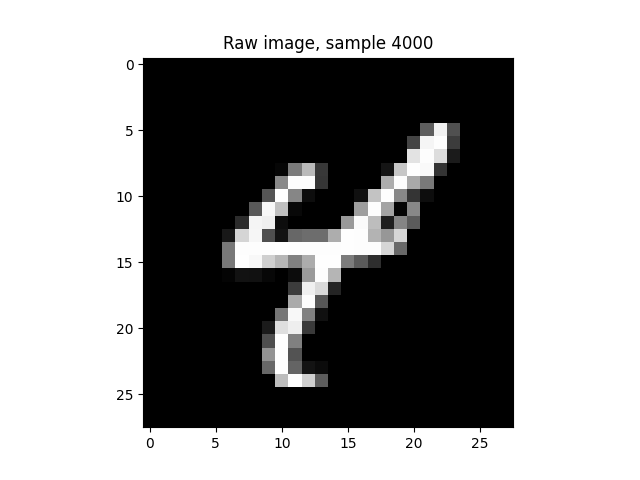
\includegraphics[width=0.35\textwidth]{image2.png}
%\captionof{figure}{Handwriting Sample 4000\label{fig:image4}}
%\end{center}    
        